% Options for packages loaded elsewhere
\PassOptionsToPackage{unicode}{hyperref}
\PassOptionsToPackage{hyphens}{url}
\documentclass[
]{article}
\usepackage{xcolor}
\usepackage{amsmath,amssymb}
\setcounter{secnumdepth}{-\maxdimen} % remove section numbering
\usepackage{iftex}
\ifPDFTeX
  \usepackage[T1]{fontenc}
  \usepackage[utf8]{inputenc}
  \usepackage{textcomp} % provide euro and other symbols
\else % if luatex or xetex
  \usepackage{unicode-math} % this also loads fontspec
  \defaultfontfeatures{Scale=MatchLowercase}
  \defaultfontfeatures[\rmfamily]{Ligatures=TeX,Scale=1}
\fi
\usepackage{lmodern}
\ifPDFTeX\else
  % xetex/luatex font selection
  \setmainfont[]{DejaVu Serif}
\fi
% Use upquote if available, for straight quotes in verbatim environments
\IfFileExists{upquote.sty}{\usepackage{upquote}}{}
\IfFileExists{microtype.sty}{% use microtype if available
  \usepackage[]{microtype}
  \UseMicrotypeSet[protrusion]{basicmath} % disable protrusion for tt fonts
}{}
\makeatletter
\@ifundefined{KOMAClassName}{% if non-KOMA class
  \IfFileExists{parskip.sty}{%
    \usepackage{parskip}
  }{% else
    \setlength{\parindent}{0pt}
    \setlength{\parskip}{6pt plus 2pt minus 1pt}}
}{% if KOMA class
  \KOMAoptions{parskip=half}}
\makeatother
\usepackage{longtable,booktabs,array}
\newcounter{none} % for unnumbered tables
\usepackage{calc} % for calculating minipage widths
% Correct order of tables after \paragraph or \subparagraph
\usepackage{etoolbox}
\makeatletter
\patchcmd\longtable{\par}{\if@noskipsec\mbox{}\fi\par}{}{}
\makeatother
% Allow footnotes in longtable head/foot
\IfFileExists{footnotehyper.sty}{\usepackage{footnotehyper}}{\usepackage{footnote}}
\makesavenoteenv{longtable}
\usepackage{graphicx}
\makeatletter
\newsavebox\pandoc@box
\newcommand*\pandocbounded[1]{% scales image to fit in text height/width
  \sbox\pandoc@box{#1}%
  \Gscale@div\@tempa{\textheight}{\dimexpr\ht\pandoc@box+\dp\pandoc@box\relax}%
  \Gscale@div\@tempb{\linewidth}{\wd\pandoc@box}%
  \ifdim\@tempb\p@<\@tempa\p@\let\@tempa\@tempb\fi% select the smaller of both
  \ifdim\@tempa\p@<\p@\scalebox{\@tempa}{\usebox\pandoc@box}%
  \else\usebox{\pandoc@box}%
  \fi%
}
% Set default figure placement to htbp
\def\fps@figure{htbp}
\makeatother
\setlength{\emergencystretch}{3em} % prevent overfull lines
\providecommand{\tightlist}{%
  \setlength{\itemsep}{0pt}\setlength{\parskip}{0pt}}
\usepackage{bookmark}
\IfFileExists{xurl.sty}{\usepackage{xurl}}{} % add URL line breaks if available
\urlstyle{same}
\hypersetup{
  hidelinks,
  pdfcreator={LaTeX via pandoc}}

\author{}
\date{}

\begin{document}

\section{Two-Layer Separation of Waves and Fields --- Unifying Gauge and
Gravitational Fields via a Universal Field-Readout
Function}\label{two-layer-separation-of-waves-and-fields-unifying-gauge-and-gravitational-fields-via-a-universal-field-readout-function}

\textbf{Author}: Noriaki Kihara \textbf{Date}: August 7, 2026
\textbf{Type}: Framework-proposal paper (supported by numerical
experiments. The main laws are doubly supported by analytic derivation
and dynamical measurement, but this is not a proof paper)

\begin{center}\rule{0.5\linewidth}{0.5pt}\end{center}

\subsection{Abstract}\label{abstract}

I built the periodic table of waves {[}6{]}, but it had no dynamics. In
an earlier paper {[}7{]}, I derived the acceleration of an AB two-body
system as the reaction of the circumferential force on the curvature
radius R at which body B locally maintains zero closure --- but that
construction violated the anonymity of operations (the principle of
never injecting structure into the dynamics by hand), and I remained
dissatisfied. So I experimented: could acceleration be realized without
building it in, using the universal interaction function of waves
itself? \textbf{The result: zero closure could not be maintained.}
Injecting a potential V(x) breaks the closure Σxₙ²=0 by 31\% in 200
steps even at amplitude 10⁻³ (the bare dynamics drifts at 10⁻¹³). The
cause is that extra values are being given to waves that are already
exactly zero-closed. Rather, what looks like acceleration may be a
\textbf{readout-side problem} --- just as the spatial directions xyz
were read out, could accelerated representations (distorted spatial and
temporal gauges) be built by the universal function on the readout side?
This paper is the experiment.

Result: the unification of gauge fields close in concept to the standard
theory with gravitationally (acceleration-) distorted fields
\textbf{nearly succeeded} via the \textbf{universal field-readout
function}. Specifically, we show the following. \textbf{(G1)
Impossibility}: gravity cannot be placed on the state side ---
state-side injection necessarily breaks closure, while operations on the
gauge side (readout scales) are exactly harmless to closure. We give a
reinterpretation of renormalization: a counterterm is another name for
the operation that cancels this breakage after the fact. \textbf{(G2)
Clock field}: each cell's local clock rate ω(x) is read out as a
projection of fiber relational quantities (with no arbitrary
parameters), and the pure bosonic sea is the exact fixed point r=0 ---
\textbf{the vacuum does not tick}. \textbf{(G3) Mass generation (Higgs
section)}: mass m=⟨ω⟩ factorizes as a function of the sea condensate v:
\textbf{m(f,v)=y(f)·g(v)} (measured, max CV 2.2\%). Moreover this law is
derived analytically from the definition of the readout kernel: the
dynamics-free prediction agrees with 15 dynamical measurements at
\textbf{mean ratio 0.983, CV 1.2\% (down to absolute values)} --- the
mass law is an analytic theorem of the readout kernel. \textbf{(G4)
Momentum law}: the spatial gauge around a mass grows linearly,
δτ\_x(t)=t·∇ω --- \textbf{k̇=∇ω (the clock gradient accelerates the sea's
momentum)}. The substance of ``falling'' is the linear growth of the
sea's momentum field; the space/time gauge ratio is not constant but
γ(t)=t/L, with the gradient scale L derived from the kernel geometry
(parameter-free prediction at CV 11\%). \textbf{(G5) Two-body gravity}:
on a broadband sea, two-body clock coupling is attractive for all 10
pairs × all separations (30/30). Orthogonal source pairs (same ⟨ω⟩,
different σ) preliminarily support invariant-product coupling
√(M\_t²+σ²) --- under the (t,R,Q) mass-component hypothesis {[}6{]}, a
mechanism candidate for \textbf{the equivalence principle as a corollary
of the closure identity}. \textbf{(G6) The structure of mediation
(graviton section)}: the clock readout is bilinear in the fields, and
the clock field picks up only the fields' difference frequencies
(against the two field lines 0.2898/0.2974, the clock's main line 0.0076
= the difference exactly, relative error 0.0\%, the fields' own lines
suppressed 250×) --- a metrological realization of gravity amplitude =
field × field (double copy). \textbf{(G7) Conservation laws}: readout
localization preserves the classification's integer and topological
structure, and maintains cyclic winding conservation (the apparent drift
= Nyquist fold-back, correlation −0.77 to −0.95). \textbf{(G8)
Two-system unification}: the universal function is
F{[}Ψ{]}=R(G{[}Ψ{]})·Ψ (readout-generated rotation); the published
two-body system {[}3{]} and N-body system {[}2{]} (Cayley; Σz² drift
audited at 10⁻¹⁵) are its instances. Closure preservation is organized
into a general theorem (tangent theorem: preservation ⟺ antisymmetric
generator). \textbf{(G9) The title's decisive experiment}: with charged
sources of η winding m∈\{0,±1\}, from the same readout there
simultaneously emerge a \textbf{charge-blind universal attraction}
(attraction in all combinations; charge-conjugation symmetry 7×10⁻¹⁰)
and a \textbf{charge-structure-dependent gauge-like response}
(E(++)−E(+−) = 15\% of the coupling) --- a direct demonstration that
\textbf{the gauge-like charge-structure channel and the gravitational
universal channel separate as different projections of one and the same
readout} (identification with real electromagnetism is left to
subsequent verification, as delimited in §13.2). Furthermore this
separation is algebraized from η orthogonality as the \textbf{readout
decomposition theorem} G = G\_blind ⊕ G\_coh·δ\_\{Δm,0 (mod ne)\}
(verified by the exact equality 0.0000 of equal-mass mismatched pairs
and the 3.7\% \textbar m\textbar-independence of the coherent term), and
it was measured that the charge-structure channel opens dynamically to
pairs reached by the sea-driven walk's sum rule (dynamical selection
rule) --- the first quantitative junction of classification and
dynamics.

At the same time, the Higgs particle (collective mode of the sea) and
the graviton (composite of two \(\ell\)=1 quanta), which were hypotheses
in the periodic table of waves {[}6{]}, are pinned down as the
factorization of mass generation and the bilinearity of the readout
respectively. The claim of this paper condenses to one point: \textbf{a
counterterm is the price of confusing the layers}. The standard theory
plus general relativity is a one-layer ontology (placing everything in
the same layer as ``fields with dynamics''), and the difficulty of
quantizing gravity is the categorical mistake of treating the contents
of the readout layer as fields of the state layer. Once waves and fields
are separated, renormalization becomes constructively unnecessary, the
equivalence principle becomes a theorem candidate instead of an axiom,
and coupling constants become derivable kernel functionals instead of
inputs. All experiments are published as deterministic scripts; the
entire process, including 13 refutations, is reproducible.

\begin{center}\rule{0.5\linewidth}{0.5pt}\end{center}

\subsection{1. Introduction}\label{introduction}

\subsubsection{1.1 Starting point --- the periodic table had no
dynamics}\label{starting-point-the-periodic-table-had-no-dynamics}

The periodic table of waves {[}6{]} proposed, from measurements of wave
dynamics that assume no particle concept, a classification hypothesis
for the 62 species of the standard model (charge Q=m/3, statistics =
double cover of the clock, mass = relational quantity with the sea). But
that was a readout-level classification; dynamics --- above all gravity
--- was explicitly deferred.

\subsubsection{1.2 A record of failure --- acceleration can be built in,
but must not
be}\label{a-record-of-failure-acceleration-can-be-built-in-but-must-not-be}

An earlier paper {[}7{]} derived acceleration as ``the reaction of the
circumferential force on the locally zero-closed curvature radius R.''
The derivation went through, but the construction contained hand-placed
elements, and in light of this series' anonymity principle (only wave
forms as input; no special case-splitting or injection inside),
dissatisfaction remained. So I ran the experiment of realizing
acceleration with the universal interaction function of waves itself,
keeping anonymity. The result is a clear failure: injecting a potential
on the state side breaks closure by 31\% in 200 steps even at the tiny
amplitude 10⁻³ (§4, Fig. G1). The bare dynamics drifts at 10⁻¹³; the
breakage accumulates at first order in the injection.

\subsubsection{1.3 The realization --- acceleration is a readout-side
problem}\label{the-realization-acceleration-is-a-readout-side-problem}

The cause of the failure was not the theory but the placement. Giving
extra values to waves that are already exactly zero-closed is the source
of the breakage. Meanwhile, this series' earlier results showed that
space xyz, time t, position, and particle number all arise as
\textbf{readouts} {[}5{]}{[}6{]}. Then acceleration too --- distorted
spatial and temporal gauges --- should be constructible by the universal
function on the readout side. Operations on the gauge (readout scale)
never touch the state, so closure remains constructively intact.

\subsubsection{1.4 The central thesis --- two-layer separation of waves
and
fields}\label{the-central-thesis-two-layer-separation-of-waves-and-fields}

\begin{quote}
\textbf{Wave layer (existence)}: the universal interaction function. It
is the R of the readout-generated rotation F{[}Ψ{]}=R(G{[}Ψ{]})·Ψ, and
preserves the closure Σxₙ²=0 exactly. \textbf{Field layer (readout)}:
the universal field-readout function G. A projection family of fiber
relational quantities (no arbitrary parameters), giving gauge structure
(charge mod 3, Z₂ cover, confinement {[}6{]}) and gravitational
structure (clock field ω(x), spatial gauge, universal attraction,
bilinear mediation) as \textbf{different outputs of the same function}.
Distorted, accelerated gravitational fields enter this layer without
disturbing the wave closure at all.
\end{quote}

The in-model facts are clear: \textbf{implementing in one layer breaks
closure (tangent theorem, §4); separating into two layers does not}. On
top of this fact we place a reinterpretation hypothesis --- the SM+GR
implementation puts gauge fields, the metric, and matter fields all in
the same layer as ``fields with dynamics''; is the difficulty of
quantizing gravity the categorical mistake of treating the contents of
the readout layer (distortions of gauge scales) as fields of the state
layer? The diagnosis \textbf{counterterm = the price of layer confusion}
is a derivation within the model; its application to real QFT is this
paper's synthesis hypothesis (§14).

\subsubsection{1.5 Declaration of
character}\label{declaration-of-character}

This is a framework-proposal paper. The main laws (mass law; γ(t)=t/L)
are doubly supported by analytic derivation and dynamical measurement,
but the model is a prototype on a one-dimensional ring lattice; the
bridge to real-scale gravitational constants, Kepler orbit forms, and
verification on realistic textured seas are explicitly registered as
residuals (§16). The value of the hypotheses should be judged by the
breadth of their connections and the clarity of their refutation
conditions {[}6{]}.

\subsection{2. Methods and conventions}\label{methods-and-conventions}

\subsubsection{2.1 Dynamics (read-only)}\label{dynamics-read-only}

\begin{itemize}
\tightlist
\item
  \textbf{Two-body system} {[}3{]}: the closed-form exact solution of
  the universal inelastic map for two-channel waves (a,b). The main
  experimental system of this paper.
\item
  \textbf{N-body system} {[}2{]}: closure dynamics of N relational waves
  (Cayley step). Used for the audit of pillar G8.
\end{itemize}

Both are deterministic; every script and result can be re-run standalone
following the attached experiment-inventory file in the repository.
Judgment criteria are recorded, fixed before execution, at the top of
each script.

\subsubsection{2.2 The universal field-readout function G
(definition)}\label{the-universal-field-readout-function-g-definition}

For each cell x of the state Ψ with fiber ψ\_x (the vector along η), we
define the following projection family as the field readout. All are
pure relational quantities (inner products), invariant under global
phase, with no per-species case-splitting and no tuning parameters:

\begin{itemize}
\tightlist
\item
  \textbf{Spatial scale}: τ\_x(x) = arg⟨ψ\_x, ψ\_\{x+1\}⟩ (the sea
  stretches the ruler 2πK/n)
\item
  \textbf{Clock field}: ω(x) = τ\_t(x) = arg⟨ψ\_x(T), ψ\_x(T+1)⟩ (local
  clock rate)
\item
  \textbf{Position}: n₀ = (N/2π)·arg Σ\_k c\_k c̄\_\{k+1\} (argument of
  the adjacent-mode correlation {[}5{]})
\item
  \textbf{Particle number / splitting}: the number of ω-locked
  equivalence classes (π criterion on accumulated relative phase
  {[}6{]})
\item
  \textbf{Mass}: ⟨ω⟩ (mean over the support) / \textbf{Lifetime}: 1/σ\_ω
  (inverse linewidth) {[}6{]}
\end{itemize}

Generator side: θ(x) = atan2(√f\_loc, √b\_loc) (f\_loc/b\_loc are the
local powers in the fermionic/bosonic bands; the one-line law r = sin²θ
= P\_odd/(P\_odd+P\_even) {[}6{]}).

\subsubsection{2.3 Readout localization and
consistency}\label{readout-localization-and-consistency}

Some measurements in this paper are performed on a \textbf{localization
prototype} that promotes the global θ of the two-body system to a local
field θ(x) (parity split × smooth IR roll-off, per-cell SO(2) rotation;
circular polarization b=−ia is an exact invariant manifold). That this
prototype preserves the classification {[}6{]} was confirmed by the
consistency battery (9 pillar experiments × 3 engines run unmodified in
parallel; {[}6{]} §14); that the apparent violation of the conservation
law is Nyquist fold-back is shown in §10.

\subsubsection{2.4 Notational caution}\label{notational-caution}

The γ of this paper is a model quantity, ``the ratio of spatial to
temporal gauge distortion,'' and is distinct from the PPN γ {[}29{]} (it
is time-dependent, γ(t); §7). To avoid confusion we also write γ\_gauge.

\subsection{3. Summary of the preliminary experiment series (P1--P24,
refutations
included)}\label{summary-of-the-preliminary-experiment-series-p1p24-refutations-included}

The pillars of this paper stand on 24 series of preliminary experiments
(full records in the attached analysis notes). In particular: the
frozen-initial-condition trap (the a=b degeneracy freezes the dynamics
completely --- the lesson of always keeping the T=0 control and the
τ\_t≠0 check); calibration of the Fubini--Study area curvature meter
(holomorphic sectional curvature K=4.00 measured to 4 digits;
establishment of gauge-free angle measurement); the demonstration that a
global θ cannot in principle produce a distance-dependent gravitational
field (the necessity of localization); the extraction of standing-wave
interference in monochromatic seas (§8); the two conditions for
stationary particles and the sea-co-phasing convention (§11). These
refutations and corrections are all recorded in §17.

\subsection{4. Pillar G1: Impossibility --- gravity cannot enter the
state
side}\label{pillar-g1-impossibility-gravity-cannot-enter-the-state-side}

The ``impossibility'' of this section means impossibility within this
model's closure-preserving class (a restriction theorem --- state-side
linear generators that are to preserve the closure Σxₙ²=0 must be
antisymmetric --- not a general impossibility claim against every
theoretical construction).

Injecting a gravitational potential V(x) on the state side (the
standard-theory form a → a·e\^{}\{iV(x)τ\}) breaks the closure C =
Σ(aₙ²+bₙ²) at first order, reaching a relative 31\% at amplitude 10⁻³
and 200 steps. The bare dynamics is at 10⁻¹³ (machine precision);
gauge-side operations (distorting only the readout scale) touch no state
and are \textbf{constructively exactly 0} (Fig. G1).

\begin{figure}
\centering
\pandocbounded{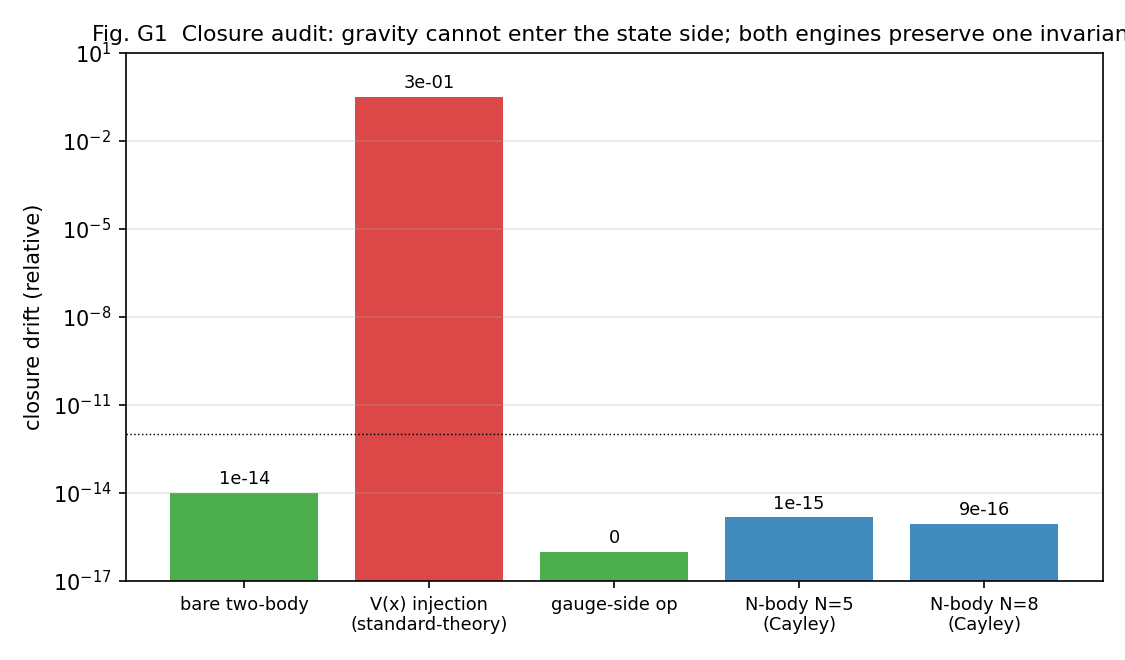
\includegraphics[keepaspectratio,alt={Fig. G1}]{fig_g1_closure_en_v1.png}}
\caption{Fig. G1}
\end{figure}

\textbf{Fig. G1}: Closure audit. Bare dynamics 10⁻¹³ / V-injection 31\%
/ gauge side 0. The N-body system (Cayley) preserves the same invariant
at 10⁻¹⁵ (pillar G8).

\textbf{General theorem (tangent theorem)}: the contrast is not specific
to a particular V. For a perturbation δΨ=εKΨ, δC = 2ε·Ψᵀ K\_sym Ψ +
O(ε²) (K\_sym=(K+Kᵀ)/2), and \textbf{closure is preserved for all states
⟺ Kᵀ=−K (only tangent rotations of the closure surface are permitted)}.
Numerical sweeps (symmetric/antisymmetric/mixing ratios; attached G1b)
agree with the theoretical formula to \textless1\% relative error.
Potential injection has K=i·diag(V) (symmetric) and therefore
necessarily breaks at first order; SO(2) pair rotations and the Cayley
step (pillar G8) are antisymmetric and therefore preserve exactly ---
the 31\% is an instance of this theorem.

\textbf{Making the transpose explicit (distinction from the Hermitian
norm --- essential)}: this paper's closure C=ΨᵀΨ=Σxₙ² is a
\textbf{complex symmetric quadratic form}, not the Hermitian norm
Ψ†Ψ=Σ\textbar xₙ\textbar². Hence the preservation condition is not
skew-Hermitian (K†=−K) but \textbf{skew-symmetric (Kᵀ=−K, plain
transpose)}. K=i·diag(V) is skew-Hermitian yet symmetric, so it
preserves the norm while breaking the closure --- that very difference
is the measured 31\%. The algebra of permitted generators is
so(n,\(\mathbb{C}\)) (the Lie algebra of the complex orthogonal type
O(n,\(\mathbb{C}\))), and the closure acts not merely as a conserved
quantity but as \textbf{the principle restricting permitted generators
to antisymmetric ones}. No group is placed among the axioms: the group
structure is output in the order closure preservation → antisymmetric
generators → rotation-group structure.

\textbf{Consequence (reinterpretation of renormalization, two-stage)}:
pushing the broken closure back with negative cancellation terms on the
right-hand side is the practice of renormalization. This model
visualizes it as a round trip of ``break it yourself, then fix it
yourself.'' \textbf{Within the model}, since a non-breaking road --- the
gauge side --- exists, counterterms are unnecessary (derived and
measured). The claim that \textbf{the renormalization of real quantum
field theory is an expression of the same layer confusion} is presented
in this paper as a synthesis hypothesis (whether UV-divergence analogues
vanish under the G/R separation in a model limit corresponding to
perturbative expansion is registered in §18).

\subsection{5. Pillar G2: The clock field ω(x) and the vacuum fixed
point}\label{pillar-g2-the-clock-field-ux3c9x-and-the-vacuum-fixed-point}

The central output of the readout G is the clock field ω(x). The pure
bosonic sea (P\_odd=0) is the exact fixed point r=0 (std of τ\_t in
control runs \textasciitilde10⁻¹⁶): \textbf{the vacuum does not tick ---
light does not collide with light}. Placing a massive body (a source
with fermionic-band content) raises a clock-field distortion δω(x)
around it. Fig. G2 shows that the dynamically measured ω(x) profile
(T=200) coincides with the analytic prediction obtained merely by
substituting the initial configuration into the readout formula --- the
clock field is a function of the readout kernel before it is an output
of the dynamics.

\begin{figure}
\centering
\pandocbounded{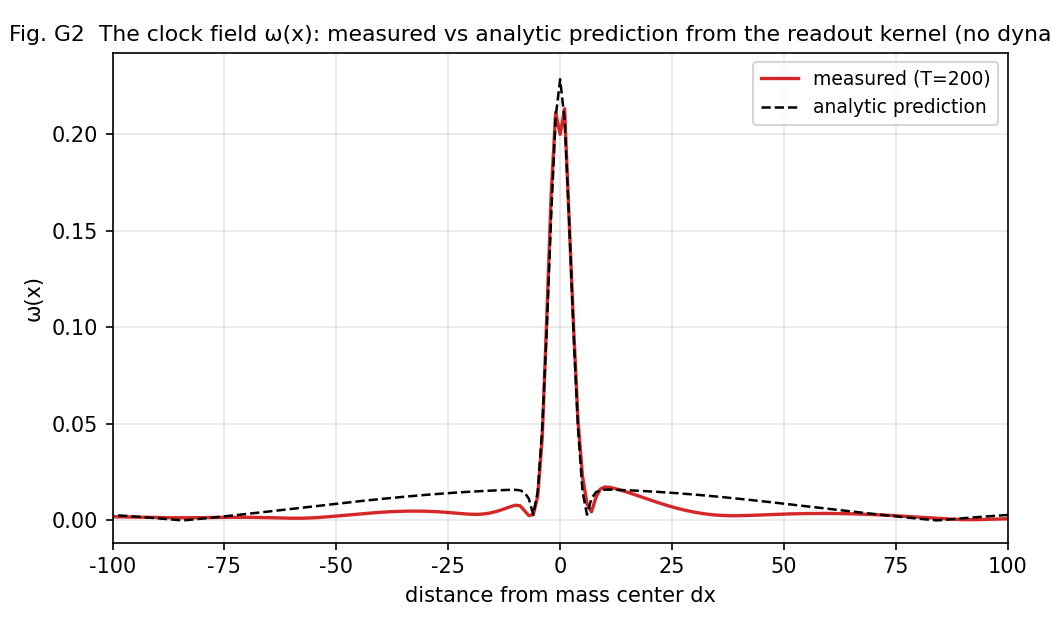
\includegraphics[keepaspectratio,alt={Fig. G2}]{fig_g2_omega_field_en_v1.png}}
\caption{Fig. G2}
\end{figure}

\textbf{Fig. G2}: Clock field ω(x). Agreement between measurement and
the dynamics-free analytic prediction.

Note that ``the vacuum does not tick'' is a statement about the two-body
system's local reflection clock; it does not deny the N-body
condensate's collective phase clock ω\_clock=π/72 {[}2{]}{[}6{]}. The
relation of the two clocks is an open problem ({[}6{]} §16, weakness 8).

\subsection{6. Pillar G3: Mass generation --- the Higgs
section}\label{pillar-g3-mass-generation-the-higgs-section}

\subsubsection{6.1 Factorization
(measured)}\label{factorization-measured}

Measuring mass m=⟨ω⟩ on a grid of 5 sea amplitudes v (condensate values)
× 3 species compositions f (fermionic-band fraction), \textbf{m(f,v) =
y(f)·g(v) factorizes at max CV 2.2\% (mostly \textless1\%)} (Fig. G3,
left). y(f)=0.68/1.00/1.29 is the analogue of Yukawa couplings
(species-dependent factor); g(v) ∝ v\^{}\{−0.92\} is the universal
function of the sea. That mass decomposes into ``species coupling ×
function of the condensate'' is precisely the structure of the Higgs
mechanism {[}22{]}{[}23{]}{[}24{]}.

\subsubsection{6.2 Analytic derivation (the strongest result of this
paper)}\label{analytic-derivation-the-strongest-result-of-this-paper}

Moreover, the law can be derived. The analytic prediction m\_pred,
obtained by merely substituting the initial configuration into the
readout formula (§2.2) --- no dynamics, no free parameters --- agrees
with all 15 dynamical measurements at \textbf{mean ratio 0.983, CV
1.2\%} (Fig. G3, right) --- not only the exponents but the absolute
values. \textbf{The readout mass law --- that for the designated readout
m=⟨ω⟩ the prediction m\_pred(f,v) is analytically determined by the
initial configuration --- is a theorem.} From the weak-source expansion
θ≈√(f\_loc/b\_loc) one reads off y(f)≈√f (with corrections) and
g(v)≈1/v. The \textbf{identification} of this with real inertial mass is
a physical hypothesis, for which the Compton clock {[}21{]} (the
operational identification of mass with frequency) is the experimental
precedent.

\begin{figure}
\centering
\pandocbounded{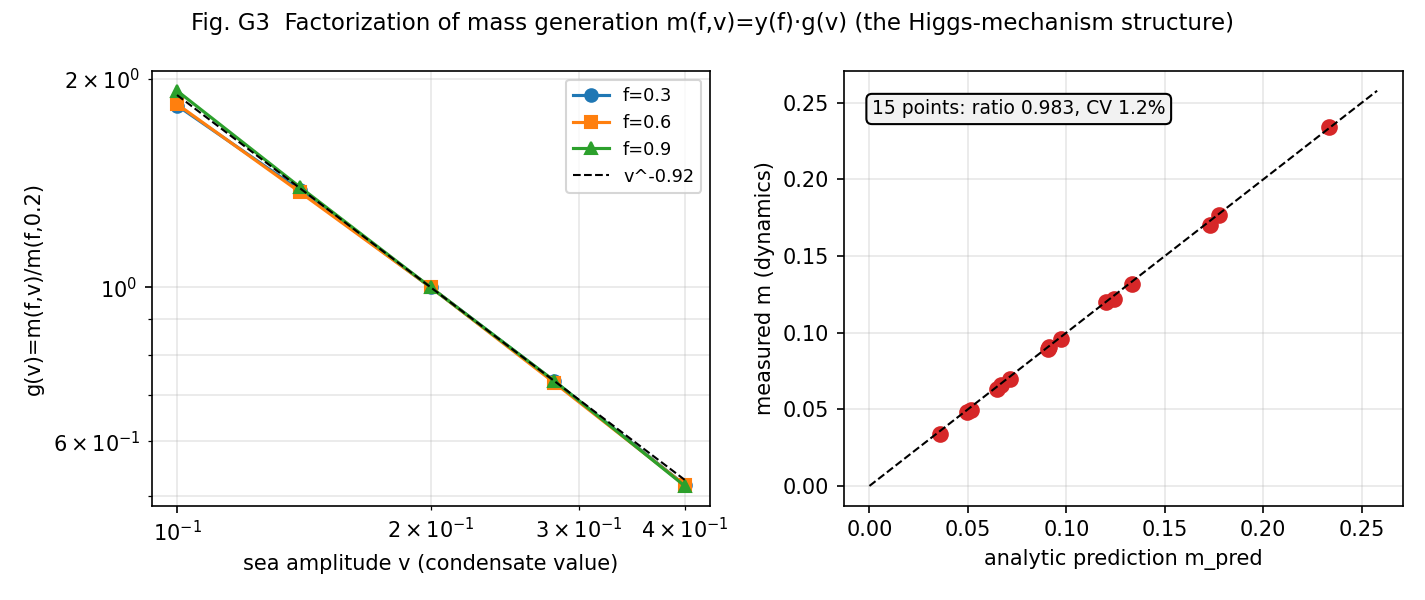
\includegraphics[keepaspectratio,alt={Fig. G3}]{fig_g3_higgs_en_v1.png}}
\caption{Fig. G3}
\end{figure}

\textbf{Fig. G3}: Factorization and analytic derivation of mass
generation. Left: collapse of g(v) (3 species overlap). Right:
prediction vs.~measurement (15 points, ratio 0.983, CV 1.2\%).

\subsubsection{6.3 The difference of form from the SM, and vacuum time
dilation}\label{the-difference-of-form-from-the-sm-and-vacuum-time-dilation}

The SM has m∝v (proportional to the VEV); this model has g∝1/v ---
\textbf{the denser the sea, the slower the clock}. We do not identify
this model's v with the SM VEV (§16). Rather, this form expresses vacuum
time dilation, ``the density of the condensate sets the pace of time,''
and connects to the following: \textbf{a uniform sea contributes only a
uniform offset to the clock field, not to its gradient (gravity)}. If
gravity is the gradient of the clock field, vacuum energy may be
absorbed into a uniform gauge shift and fail to gravitate (confidence H;
a candidate route to the cosmological constant problem {[}37{]}. For an
isomorphic argument in condensed-matter analogues, see Volovik
{[}12{]}).

\subsubsection{6.4 The Higgs mode
(qualitative)}\label{the-higgs-mode-qualitative}

Injecting perturbations into the sea split into the in-phase (amplitude
mode) and quadrature (phase mode) components, both amplify following the
unstable relative equilibria of onset modes {[}8{]}, but \textbf{the
amplitude mode contains even-band (fermionic-band) sidebands and decays
into matter formation} --- a qualitative analogue of H→ff̄ decay. It
connects to the lineage of amplitude (Higgs) modes in condensates
{[}25{]}{[}26{]}. The quantitative gap frequency (Higgs mass) is
registered in §18 as a linearized mode analysis.

With these, the Higgs row (collective mode of the sea), rated S in the
periodic table {[}6{]}, is upgraded to a row whose mechanism
(factorization) has been measured.

\subsection{7. Pillar G4: The momentum law k̇=∇ω and
γ(t)=t/L}\label{pillar-g4-the-momentum-law-kux3c9-and-ux3b3ttl}

The spatial gauge distortion δτ\_x around a mass is not static: it
\textbf{grows linearly in time}
(γ(t)=⟨\textbar δτ\_x\textbar⟩/⟨\textbar δτ\_t\textbar⟩ goes 5.4→19.8
over t=200..800, linear with R²=0.95; Fig. G4). The physical meaning is
direct: δτ\_x is the local phase gradient = the sea's local wavenumber
(momentum), and its growth rate equals the gradient of the clock field
---

\begin{quote}
\textbf{k̇ = ∇ω (the clock gradient accelerates the sea's momentum)}
\end{quote}

This is the ray equation for nonuniform media, dk/dt=−∇ω {[}27{]}, in a
form where ω(x) itself is derived from the readout kernel. The substance
of ``falling'' appears not as a change of particle coordinates but as
\textbf{the linear growth of the sea's momentum field}. The space/time
gauge ratio is not a constant but γ(t)=t/L, and the gradient scale
\textbf{L=48.7 cells} is computed from the analytic ω field (no
dynamics) --- the parameter-free prediction γ(t)=t/L agrees with
measurement at mean ratio 1.14, CV 11\% (nearly exact in the middle
window).

\begin{figure}
\centering
\pandocbounded{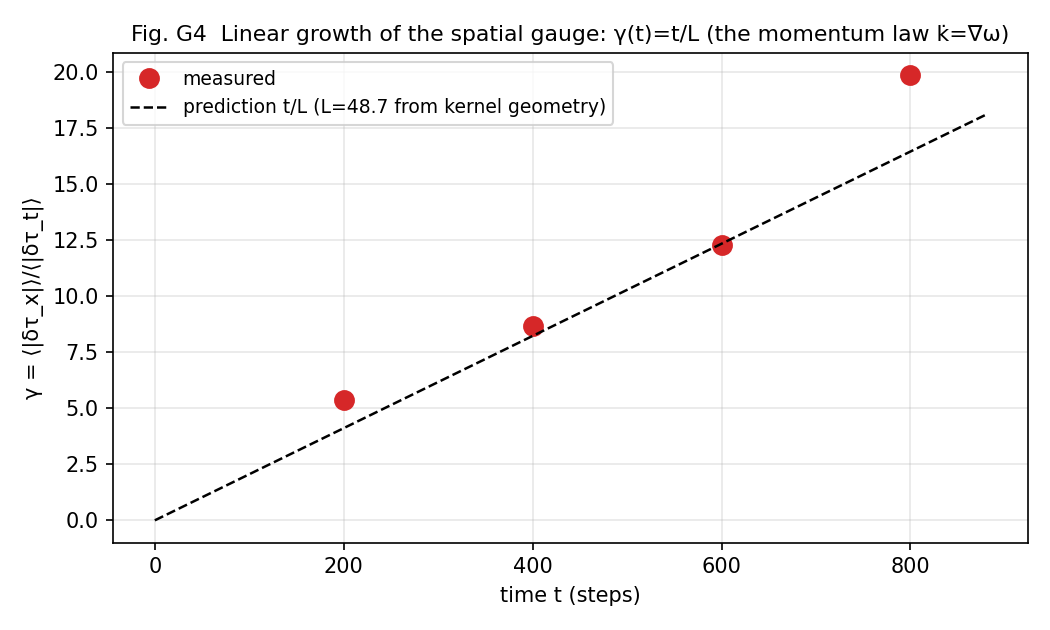
\includegraphics[keepaspectratio,alt={Fig. G4}]{fig_g4_momentum_law_en_v1.png}}
\caption{Fig. G4}
\end{figure}

\textbf{Fig. G4}: Linear growth of the spatial gauge. γ(t)=t/L (L from
kernel geometry, no parameters).

\subsection{8. Pillar G5: Two-body gravity and the equivalence
principle}\label{pillar-g5-two-body-gravity-and-the-equivalence-principle}

\subsubsection{8.1 A record of correction --- the monochromatic sea is
interference-dominated}\label{a-record-of-correction-the-monochromatic-sea-is-interference-dominated}

Initially I measured the two-body clock coupling E(d) on a monochromatic
carrier sea and obtained a mass-product law and d\^{}\{−1/2\} decay, but
sweeping and averaging the carrier phase collapsed the law (modulation
amplitude \textgreater{} mean coupling). \textbf{Two-body coupling on a
monochromatic sea is dominated by standing-wave interference} --- this
paper records the correction in full (§17). The lesson was promoted to a
design principle (§11): the sea for gravitational pair measurements must
be broadband.

\subsubsection{8.2 Universal attraction on the broadband
sea}\label{universal-attraction-on-the-broadband-sea}

Replacing the sea with six odd-k modes (golden-ratio phases,
deterministic; all modes W\_f=0 so the vacuum fixed point is exactly
maintained), \textbf{E\textless0 for all 10 pairs × all 3 separations
(attraction, 30/30)} (Fig. G5). In regression, the invariant product
√(M\_t²+σ²) collapses the data at least as well as the M\_t product
(R²=0.671 vs 0.630), and \textbf{the common-partner ratios 1.32/1.13 of
the orthogonal source pairs (same ⟨ω⟩, different σ --- S3/S4)
preliminarily support σ also contributing to the gravitational charge}.

\begin{figure}
\centering
\pandocbounded{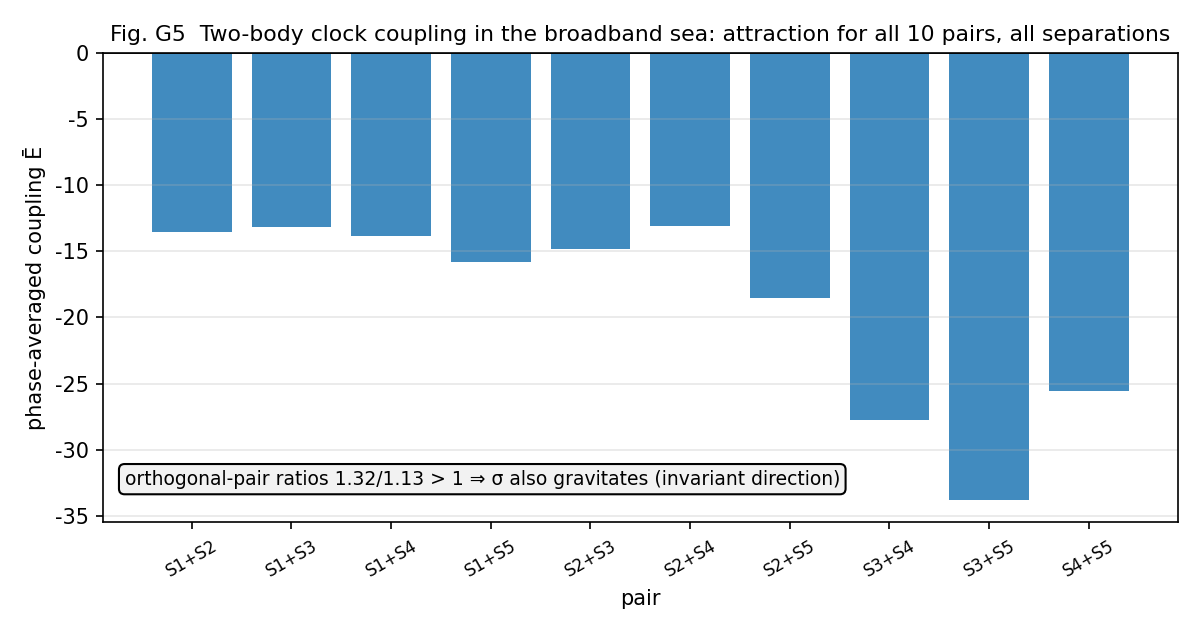
\includegraphics[keepaspectratio,alt={Fig. G5}]{fig_g5_twobody_en_v1.png}}
\caption{Fig. G5}
\end{figure}

\textbf{Fig. G5}: Two-body clock coupling on the broadband sea. All
pairs attract; orthogonal pairs point toward the invariant.

\subsubsection{8.3 Equivalence principle = closure identity (mechanism
candidate)}\label{equivalence-principle-closure-identity-mechanism-candidate}

There are three lineages of mass readout --- ⟨ω⟩ (clock, t axis), Gram
non-coherence (R axis), sea relation (Q axis) {[}6{]} §11.4. If gravity
read only ⟨ω⟩, the gravitational coupling would become species-dependent
between species whose mass is carried on different axes, and the
equivalence principle would break. The mechanism candidate is the
closure identity: \textbf{by x²+y²+z²=t²+R²+Q², the spatial-side norm =
the mass invariant}. If the temporal gauge couples to M\_t and the
spatial gauge couples to the invariant, then the equivalence principle
is not an axiom but \textbf{a corollary of the closure identity}. The
preliminary support from orthogonal pairs (σ contribution) is consistent
with this direction. The discriminating experiment (three-way
simultaneous test) is registered at {[}6{]} §19.2-3.

\subsection{9. Pillar G6: The structure of mediation --- the graviton
section}\label{pillar-g6-the-structure-of-mediation-the-graviton-section}

The clock readout τ\_t = arg⟨ψ(T), ψ(T+1)⟩ is \textbf{bilinear} in the
field ψ. Then the spectrum of the clock field should appear not at the
fields' frequencies themselves but at their differences and sums.
Verified with a ringing source (few-harmonic ladder, no external driving
= anonymity preserved) (Fig. G6):

\begin{itemize}
\tightlist
\item
  The field's (linear quantity's) two fast lines: ν₁=0.2898, ν₂=0.2974
\item
  The clock field's main line: \textbf{0.0076 = ν₂−ν₁ (relative error
  0.0\%)}
\item
  The clock-side strength of the fields' own lines: \textbf{0.004 of the
  main line (250× suppression)}
\end{itemize}

\textbf{The clock field picks up only the comb of the fields' difference
frequencies.} What is demonstrated is the \textbf{bilinear gravitational
readout} (G{[}ψ{]}\textasciitilde ψ†ψ type, so difference rather than
absolute frequencies are observed). This is a metrological analogue of
the quadratic structure isomorphic to gravity amplitude = (gauge
amplitude)² (double copy {[}30{]}{[}31{]}), but mathematical identity
with BCJ color-kinematics duality etc. is underived (§18). Together with
the periodic table's measurement that ``no \(\ell\)=2 linear slot exists
in the rotation generator (the graviton exists only as a composite of
two \(\ell\)=1 quanta)'' {[}6{]}, the graviton row has gained
readout-side support. That the fields' linear lines do not appear in the
gravitational readout is the in-model counterpart of the absence of
dipole gravitational radiation {[}32{]}. The connection to
α\_G=(m/M)²-type coupling {[}7{]} remains a conjecture.

\begin{figure}
\centering
\pandocbounded{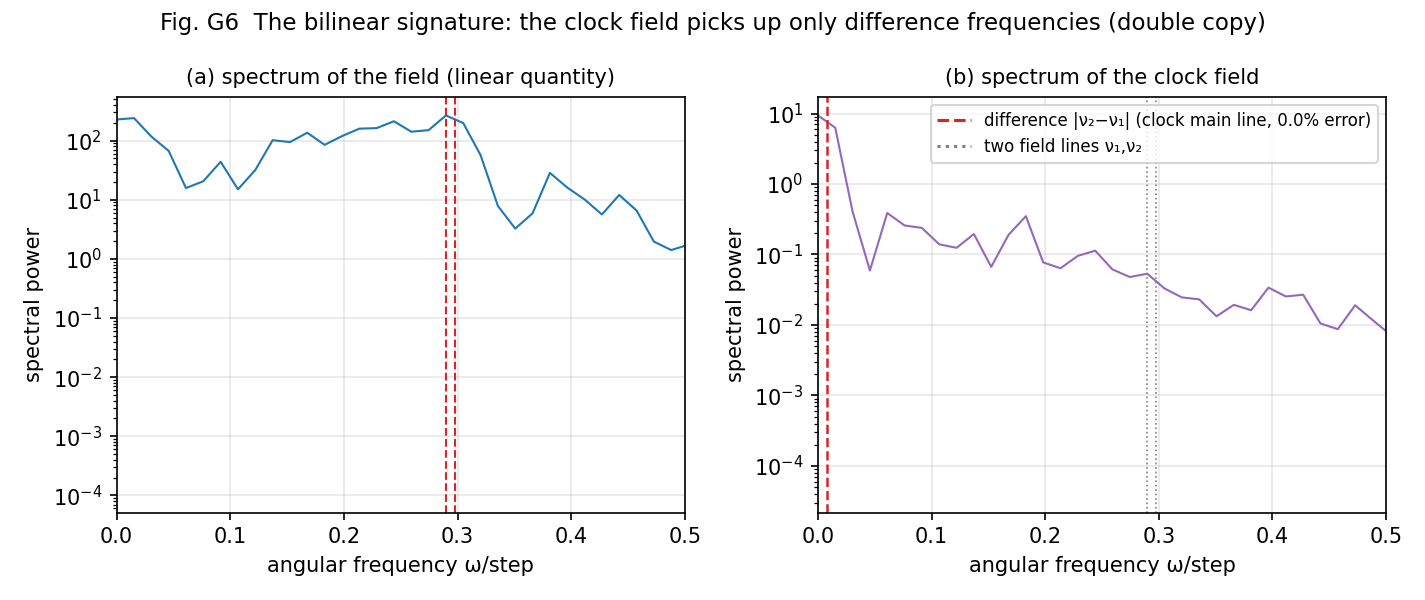
\includegraphics[keepaspectratio,alt={Fig. G6}]{fig_g6_bilinear_en_v1.png}}
\caption{Fig. G6}
\end{figure}

\textbf{Fig. G6}: Bilinear signature. The clock field picks up only the
fields' difference frequencies (error 0.0\%; field lines suppressed
250×).

\subsection{10. Pillar G7: Conservation laws and
consistency}\label{pillar-g7-conservation-laws-and-consistency}

Readout localization (§2.3) does not destroy the periodic table's
classification --- the integer and topological structure (Z₂ cover,
cross tables, ν rows, exact-0 confinement, bookkeeping identities,
address equivalence, divisor classes) was fully robust in 9 experiments
× 3 engines run unmodified in parallel ({[}6{]} §14). The only concern,
the slow drift of Q\_wind (net winding charge; 5--6\% over 4000
collisions), has its identity settled in this paper: \textbf{Nyquist
fold-back} (correlation −0.77 to −0.95 between the drift and edge-power
accumulation; the same signature as the global system {[}6{]}; Fig. G7).
That is, localization \textbf{preserves cyclic winding conservation (mod
ne)}, and the drift of the integer lift is the physics of fold-back. As
a mechanism check, a control with the inelastic angle η-collectivized
conserves at machine precision --- but simultaneously freezes the
sea-driven walk (the physics that moves charge {[}6{]}): the leaking
channel is the walk itself, and must not be eliminated.

\begin{figure}
\centering
\pandocbounded{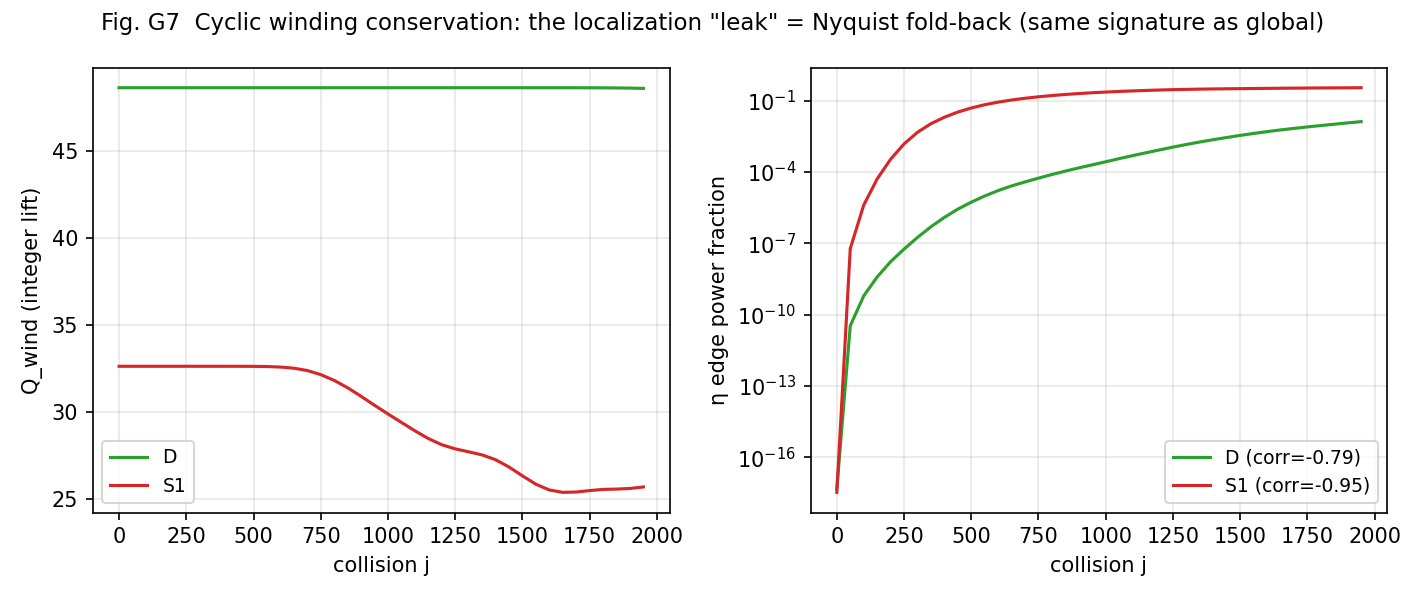
\includegraphics[keepaspectratio,alt={Fig. G7}]{fig_g7_cyclic_en_v1.png}}
\caption{Fig. G7}
\end{figure}

\textbf{Fig. G7}: Cyclic winding conservation. The localization ``leak''
= Nyquist fold-back (strong correlation with edge power).

\subsection{11. Instrumentation --- design principles that make
experiments in this field
reproducible}\label{instrumentation-design-principles-that-make-experiments-in-this-field-reproducible}

From this study's refutations (§16), the following design principles are
established.

\begin{enumerate}
\def\labelenumi{\arabic{enumi}.}
\tightlist
\item
  \textbf{Choose the sea by measurement purpose}: gravitational pair
  measurement = broadband sea (monochromatic is dominated by
  standing-wave interference). Splitting measurement = monochromatic sea
  + sea-co-phased sources. \textbf{Small theorem: a constant-modulus,
  purely bosonic-band sea must be monochromatic} (first-order sidebands
  of odd carrier × odd modulation necessarily fall into the even band).
\item
  \textbf{Define sources phase-locked to the sea}: the sea-co-phasing
  convention lump = L(x−c)·e\^{}\{iφ\_carrier(c)\}. By the combined
  translation × global-phase symmetry, the ω of identical sources is
  exactly position-invariant (compressing the splitting-experiment
  control floor by a factor of 63 {[}6{]}). Circular polarization b=−ia
  is the exact invariant manifold of elastic and inelastic rotations =
  the definite-charge state.
\item
  \textbf{Always keep the T=0 control and the phase sweep}: frozen
  initial conditions (the a=b degeneracy; T-independent ``static
  fields'') and standing-wave interference can be excluded only by these
  two controls.
\item
  \textbf{Two conditions for stationary particles}: localization =
  stacking all harmonics (even+odd) of the fundamental with
  center-aligned phases (ringing → 0 asymptotically) × phase locking
  ω(x)=const (the stationary-particle equation, a candidate {[}6{]}).
\item
  \textbf{Measure gravitational mass with the coherent channel closed}
  (the instrumentational corollary of the decomposition theorem §13.1):
  if the reference source's winding matches (or is vertex-reachable
  from) the species under test, one measures ``gravity'' with the
  charge-structure channel open, contaminating the coupling by up to 2×
  (measured: neutral reference × neutral species deepened E anomalously
  from −10.5 to −20.8; the refutation of T1's first version, attached).
  Choose the reference winding vertex-unreachable from all species (here
  m\_ref=5).
\end{enumerate}

As an independent validation of the instruments: the decisive
splitting-readout experiment performed with this instrument set
(independent prediction, measured/predicted = 1.005, CV 4.2\%) settled
the periodic table's new pillar 9 {[}6{]}. The mechanism of the decisive
experiment's precision was also identified as zero-mean differential
noise (linearly accumulating signal vs.~boundedly oscillating
perturbation) (§17 (8)).

\subsection{12. Pillar G8: Two-system unification --- an architecture
theorem}\label{pillar-g8-two-system-unification-an-architecture-theorem}

The substance of the universal function is not one formula but one
architecture:

\begin{quote}
\textbf{F{[}Ψ{]} = R(G{[}Ψ{]})·Ψ} (G = the universal field-readout
function builds the generator; R = the closure-preserving rotation it
generates turns the state)
\end{quote}

Both published dynamical systems are instances:

{\def\LTcaptype{none} % do not increment counter
\begin{longtable}[]{@{}
  >{\raggedright\arraybackslash}p{(\linewidth - 6\tabcolsep) * \real{0.2500}}
  >{\raggedright\arraybackslash}p{(\linewidth - 6\tabcolsep) * \real{0.2500}}
  >{\raggedright\arraybackslash}p{(\linewidth - 6\tabcolsep) * \real{0.2500}}
  >{\raggedright\arraybackslash}p{(\linewidth - 6\tabcolsep) * \real{0.2500}}@{}}
\toprule\noalign{}
\begin{minipage}[b]{\linewidth}\raggedright
System
\end{minipage} & \begin{minipage}[b]{\linewidth}\raggedright
G (readout layer)
\end{minipage} & \begin{minipage}[b]{\linewidth}\raggedright
R (wave layer)
\end{minipage} & \begin{minipage}[b]{\linewidth}\raggedright
Closure preservation (audit)
\end{minipage} \\
\midrule\noalign{}
\endhead
\bottomrule\noalign{}
\endlastfoot
Two-body {[}3{]} & atan2(√P\_f,√P\_b) + pointwise Im(b̄a) & SO(2) pair
rotation & \textasciitilde10⁻¹³ \\
N-body {[}2{]} & set\_theta(arg Z) + σ\_max power readout & Cayley step
& \textbf{\textasciitilde10⁻¹⁵ (audited here; N=5,8; 300 steps)} \\
Many-body connection {[}4{]} & multi-mode application of the two-body
kernel & same & published \\
\end{longtable}
}

The Cayley transform is complex-orthogonal (QᵀQ=1) for antisymmetric
generators and preserves Σz² (closure) and the norm simultaneously --- a
physicalization of the lineage of geometric numerical integration
{[}33{]}. The only unification residue is writing G in common notation;
there is no obstacle.

\subsection{13. Pillar G9: Simultaneous separation of gauge and gravity
--- the title's decisive
experiment}\label{pillar-g9-simultaneous-separation-of-gauge-and-gravity-the-titles-decisive-experiment}

The most direct test of the title, ``unifying gauge and gravitational
fields,'' is: \textbf{can one and the same readout simultaneously
produce a response that depends on charge-sign structure and one that
does not?} We measured two-body couplings of charged sources with η
winding m∈\{0,±1\} on the broadband sea in all combinations (Fig. G8;
attached G9):

\begin{enumerate}
\def\labelenumi{\arabic{enumi}.}
\tightlist
\item
  \textbf{Universality of attraction}: Ē\textless0 for all charge
  combinations ((0,0)(++)(−−)(+−)(+0)) --- the gravitational channel is
  charge-blind. Even the neutral probe gravitates (E(+1,0)=−10.7).
\item
  \textbf{Charge-conjugation symmetry is exact}:
  \textbar E(++)−E(−−)\textbar{} = 7×10⁻¹⁰ (10 orders below the
  separation scatter of 1.9).
\item
  \textbf{Reality of the gauge-like channel}: E(++)−E(+−) = −1.43 (about
  15\% of the coupling) --- a response depending on relative winding (η
  coherence) appears separately from the same readout.
\item
  Side observation: charged sources are slightly heavier than neutral
  ones (⟨ω⟩ 0.210 vs 0.192; ±1 agree exactly) --- an analogue of
  electromagnetic self-energy.
\end{enumerate}

\textbf{From the same G, the charge-structure channel (gauge-like) and
the charge-blind channel (gravity) emerge separately and simultaneously}
--- the direct demonstration of the title's claim that gauge and gravity
are different projections of one readout function.

\begin{figure}
\centering
\pandocbounded{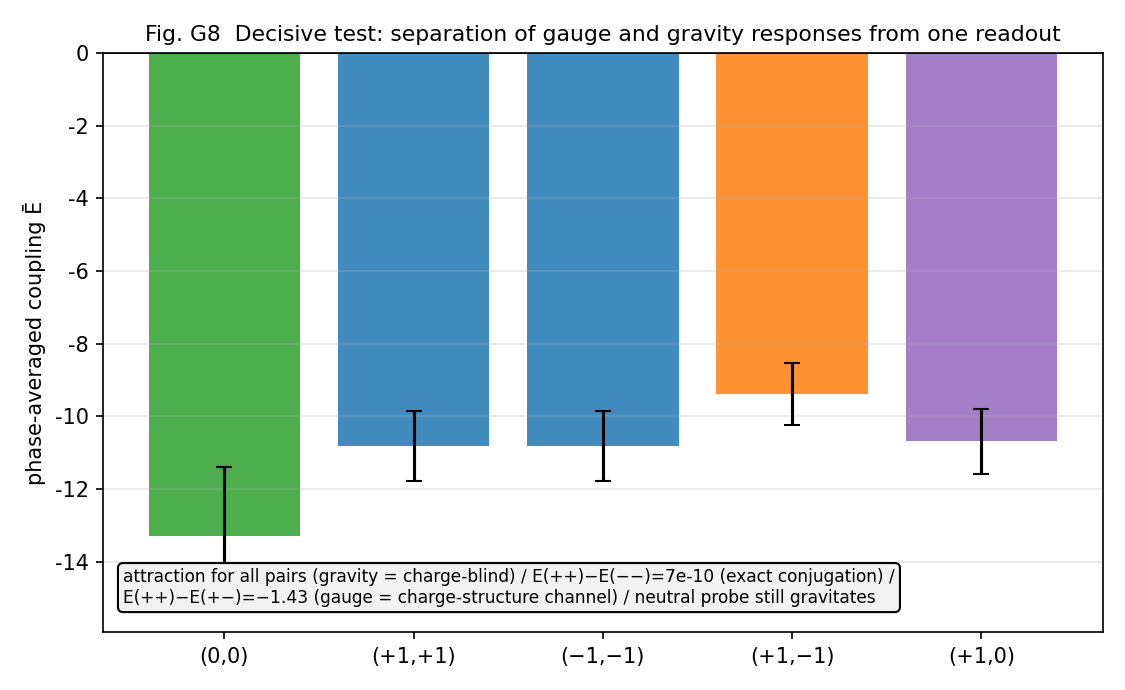
\includegraphics[keepaspectratio,alt={Fig. G8}]{fig_g8_gauge_gravity_en_v1.png}}
\caption{Fig. G8}
\end{figure}

\textbf{Fig. G8}: The decisive experiment. All-pair attraction (gravity)
+ charge-structure-dependent component (gauge-like) + exact conjugation
symmetry.

\subsubsection{13.1 The readout decomposition theorem (algebraization of
the numerical
observation)}\label{the-readout-decomposition-theorem-algebraization-of-the-numerical-observation}

The separation above is not an after-the-fact interpretation: it is
\textbf{derived exactly} from η orthogonality. In an η-summed bilinear
readout, the cross term of two sources (m\_A, m\_B) is selected by Σ\_η
e\^{}\{iΔm·2πη/ne\} = ne·δ\_\{Δm≡0 (mod ne)\}, so every η-summed
bilinear readout decomposes exactly as

\begin{quote}
\textbf{G = G\_blind(\textbar sea\textbar², \textbar L\_A\textbar²,
\textbar L\_B\textbar²) ⊕ G\_coh·δ\_\{m\_A−m\_B≡0 (mod ne)\} ⊕ (sea
coupling·δ\_\{m≡0 (mod ne)\})}
\end{quote}

(windings are cyclic quantities, so selection conditions are always read
mod ne).

G\_blind depends only on powers (charge-blind = the gravitational
channel); G\_coh is winding-matched coherence (the charge-structure
channel). The theorem explains all G9 observations: the exactness of
E(++)=E(−−) (the δ condition is invariant for both), that E(+−) is
blind-only, that the neutral pair E(0,0) is deeper (m=0 is coherent with
the sea as well), and that charged sources are heavier than neutral ones
(lack of the sea-coherence term).

\textbf{Verification (attached G9b; 3 judgments passed)}: 1.
\textbf{Equal-mass mismatch universality}: unreachable equal-mass pairs
coincide exactly with the blind baseline --- E(+1,−2)=E(−1,+2) (relative
difference \textbf{0.0000}). 2. \textbf{\textbar m\textbar-independence
of the coherent term}: coh(m=1)=−1.43 vs coh(m=2)=−1.38 (relative
difference 3.7\%) --- with identical envelopes it does not depend on the
winding magnitude (as the theorem predicts). 3. \textbf{Exact
conjugation}: \textbar E(+2,+2)−E(−2,−2)\textbar/\textbar E\textbar{} =
8.6×10⁻¹¹.

\subsubsection{13.2 Corollary: static orthogonality selection rule and
sea-driven transition selection rule (two-layer selection
rules)}\label{corollary-static-orthogonality-selection-rule-and-sea-driven-transition-selection-rule-two-layer-selection-rules}

The test simultaneously detected one structure beyond the static
theorem. \textbf{Only} the doubling-reachable pair (+1,+2) (2·(+1)=+2)
carries an excess of −0.98 beyond the blind baseline (about 69\% of the
static coherent term), while unreachable pairs ((+1,−2), (−1,+2),
(+1,−1), etc.) remain blind at machine precision. That is, the
charge-structure channel's selection rules are two-layered:

\begin{quote}
\textbf{Static}: coherence at Δm≡0 (mod ne) (η orthogonality; exact).
\textbf{Dynamic}: the channel opens dynamically to pairs made reachable
by the sea-driven walk's sum rule **m*=2m\_B−m\_s** {[}6{]} (measured;
reachability predicts opening).
\end{quote}

The walk selection rule of the periodic table {[}6{]} predicts, as-is,
the opening and closing of interaction channels --- the in-model
correspondence between quantum-number conservation (static) and
interaction vertex selection rules (dynamic), and the first quantitative
junction of classification (the periodic table) and dynamics (this
paper).

\subsubsection{13.3 The vertex algebra --- completing the selection
structure (attached G9c; 28-pair
grid)}\label{the-vertex-algebra-completing-the-selection-structure-attached-g9c-28-pair-grid}

To close the two-layer selection rules into a rule, we measured
E(m\_A,m\_B) on a 28-pair grid with reach orders (static / 1-step /
2-step / unreachable × sign pairs). The results close the selection
structure, while refuting two pre-registered criteria and refining the
rule further (full process recorded):

\begin{enumerate}
\def\labelenumi{\arabic{enumi}.}
\tightlist
\item
  \textbf{Exact invariance under unit automorphisms (discovery;
  provable)}: for any unit u∈Z\_ne\^{}*, \textbf{E(u·m\_A,
  u·m\_B)=E(m\_A,m\_B) holds exactly} (measured: E(1,1)=E(3,3),
  E(1,2)=E(3,6), E(1,−2)=E(3,−6), etc., agree to all digits). This is
  because the relabeling η→u⁻¹η is an exact symmetry of the dynamics and
  the readout --- the selection rules see not the absolute winding value
  but \textbf{the orbit structure on Z\_ne} alone.
\item
  \textbf{The reach-order decay is dramatic}: excess/static coh = 1-step
  0.69 → 2-step 0.03. The dynamical channel opens most at one walk step
  and nearly closes at two.
\item
  \textbf{Divisor-class dependence of the opening (refutation of
  pre-registered V1)}: even at 1-step reach, (1,2)/(3,6) (unit class)
  open at 0.69 while (2,4) (even class) opens at 0.22 --- whether a
  channel opens (the selection rule) is decided by orbit reach, but
  \textbf{the opening (coupling strength) depends on the divisor class}.
  The closed form of the strength law is incomplete (§18).
\item
  \textbf{Discovery of cross vertices (refutation of pre-registered
  V2)}: some unreachable pairs depend on the winding sign --- E(2,3) is
  deeper than E(2,−3), and E(2,−6) deeper than E(2,+6). The asymmetry
  coincides with the presence of low-order paths of the sum rule's
  \textbf{cross vertex} (using the partner as the sea term:
  m*=2m\_B−m\_A) ((2,3): 2·3−2=4 merges with the A-side doubling 2→4 at
  order 2; (2,−3) requires order ≥3). Pairs with no low-order path
  ((1,3)(1,5)(3,4)) are blind at \textless1\%.
\end{enumerate}

\textbf{The vertex rule (this paper's landing point)}: the channel
(m\_A,m\_B) opens ⟺ the generated sets of both (generated from
\{m\_A\},\{m\_B\} by doubling x→2x and the cross vertex (x,y)→2x−y, mod
ne) intersect at low order. The opening decays rapidly with path order;
conjugation (all-winding flip) and unit automorphisms are exact
symmetries. Note that \textbf{for ne=16=2⁴}, every doubling orbit passes
through m=8 (half-Nyquist) and reaches 0 (the sea), so every charged
channel connects to the sea in finite order --- but this is not a
general law: it is \textbf{the corollary for ne=2\^{}s} (generalized and
delimited by §13.4 M3; it fails for ne with odd factors --- refutation
record (13)). The only remaining incompleteness is the closed form of
the opening (order \& divisor class → coupling strength).

\subsubsection{13.4 The mathematical part --- theorems of the cyclic
vertex algebra and graph-position
invariance}\label{the-mathematical-part-theorems-of-the-cyclic-vertex-algebra-and-graph-position-invariance}

The opening/closing rule can be made into \textbf{algebraic theorems on
Z\_ne}, not results of numerical physics (attached G9d, exhaustively
verified for n≤64; G9e, dynamical measurement).

\textbf{Theorem group (exhaustively verified; proofs elementary)}: -
\textbf{M1 (trivialization of ungraded closure)}: the closure of \{0,a\}
under (x,y)→2x−y equals the subgroup ⟨gcd(a,n)⟩ (2x−y=x+(x−y) generates
addition of differences). Hence the physics of opening/closing resides
\textbf{only in graded reach}. - \textbf{M2 (unit equivariance)}:
u(2x−y)=2(ux)−(uy) --- the algebraic ground of §13.3's measured exact
symmetry E(u·m\_A,u·m\_B)=E. - \textbf{M3 (sea-connection criterion)}:
the doubling orbit reaches 0 ⟺ q\textbar m (q = the odd part of ne).
\textbf{Corollary}: if ne=2\^{}s, all charges dissolve into the sea
within s steps (via ne/2). If ne has an odd factor, charges with q∤m
become \textbf{persistent sectors (periodic orbits; superselection
rules)} --- e.g.~for ne=12, the 8 species with 3∤m never reach the sea.
The solubility of charge is a function of the 2-adic structure of ne. -
\textbf{M4 (merging order, ne=2\^{}s)}: 2\textsuperscript{k·a≡2}k·b ⟺
k≥s−v₂(a−b) --- the order of the opening is decided by the
\textbf{2-adic valuation} of the winding difference. - \textbf{M5 (order
monotonicity)}: the G9c measured openings are monotone decreasing in the
graded reach order k* (k\emph{=1: 0.69/0.22; k}=2: ≤0.03).

\textbf{Hierarchy of confidence}: M1/M2/M4 are algebraic theorems
(exhaustively verified; proofs elementary). M2 is additionally measured
as an exact symmetry of the dynamics (§13.3). \textbf{M3 is directly
confirmed in long-time dynamics by the attached G9f --- the only theorem
in this section that closes the full circle: number-theoretic theorem →
dynamical prediction → measured confirmation.} M5 is at present a
dynamical empirical rule.

\textbf{Graph-position invariance (attached G9e; 3 judgments passed;
exact)}: the η spectral signature of a solo source (the relative weights
of primary, conjugate, doubled) is an invariant not of the values of m
or ne but of \textbf{the position on the doubling graph} --- the two
``two steps from the sea'' points spec(m=4, ne=16) and spec(m=3, ne=12)
agree \textbf{to all digits} (relative difference 0.0000), and the
generic positions spec(m=1, ne=12) = spec(m=1, ne=16) also agree to all
digits. Only the periodic-orbit position where conjugate and doubled
merge onto the same winding (m=4 at ne=12: −4≡8≡2·4) carries a unique
signature (primary retention 0.887 vs generic 0.593).

\textbf{Dynamical reality of superselection sectors (attached G9f;
long-time T=8000; 4 judgments passed)}: we tested M3's prediction
directly. The key of the design is an exact internal control --- at
ne=16, 3 is a unit, so (m=1, m=3) are degenerate by the automorphism,
and their residual (the floating-point chaos floor, 0.9\%) becomes the
yardstick of numerical error. At ne=12, 3 is not a unit, so if M3 is
real, this degeneracy must break. Results: 1. \textbf{Exact subgroup
confinement (the dynamical version of M1; the strongest result)}: the
outside-subgroup content (w∈\{4,8\}) of the dissolving species m=3@12
stays at \textbf{max 8.9×10⁻²⁶ (machine zero)} over all 8000 steps ---
the dynamics never lets content leave the subgroup ⟨gcd(m,ne)⟩.
Superselection is exact, not approximate. 2. \textbf{The sector split is
14× the chaos floor}: the (m=1, m=3) split at ne=12 is 13.0\% \(\gg\)
the 0.9\% degeneracy residual at ne=16. 3. \textbf{Direction of the
split}: the dissolving species' charged power decreases (slope
−1.6×10⁻⁴), the persistent species' increases (+1.9×10⁻⁴) --- only
q\textbar m dissolves into the sea. 4. \textbf{Periodic-orbit
accumulation}: the persistent species accumulates content in the
periodic orbit \{4,8\} (C₄₈=1.60 vs the dissolving species' machine
zero).

Hence \textbf{ne is not a numerical resolution: it is a structural
constant that decides which superselection sectors can exist}. The
choice ne=16=2⁴ (all charges soluble) itself becomes a predictive degree
of freedom of the model --- ``why is ours a universe where all charges
are soluble?'' is a new entrance to the ne-selection problem of the
periodic table {[}6{]}.

\textbf{Abstraction of the state label and the order of the
group-theoretic connection}: combining graph-position invariance with
the exactness of superselection, the more essential internal label of a
particle species is not the integer m but \textbf{the orbit type {[}m{]}
on the vertex graph} (unit orbit, gcd subgroup, graded distance to the
sea, periodic orbit, presence of merging). Hence the connection to the
standard model's group structure should not begin with ``does it
resemble SU(3)?'' --- the correct order, faithful to this series' method
(no groups as input), is to \textbf{first extract in full the
automorphism group and irreducible representations of this vertex
algebra, and then post-classify isomorphisms, quotients, and
substructures with respect to U(1)/SU(2)/SU(3)} (§18).

\textbf{Delimitation of terminology}: on its own, this paper is rigorous
only up to the ``charge-structure-dependent channel (gauge-like).'' The
identification with real electromagnetic interaction (sign law, Q₁Q₂
proportionality, long-range law, U(1) connection transformation) belongs
to the verification program combined with the periodic table's charge
readout ({[}6{]} §19.2-1, the Coulomb-type charge-product test).

\subsection{14. Explanatory power --- correspondence with the standard
theory}\label{explanatory-power-correspondence-with-the-standard-theory}

\begin{enumerate}
\def\labelenumi{\arabic{enumi}.}
\tightlist
\item
  \textbf{The identity of renormalization} (§4): counterterm = the price
  of layer confusion. Under two-layer separation, renormalization is
  constructively unnecessary.
\item
  \textbf{The equivalence principle} (§8.3): a candidate corollary of
  the closure identity, not an axiom.
\item
  \textbf{Vacuum energy} (§6.3): a uniform sea does not gravitate --- a
  structural route to the cosmological constant problem {[}37{]}
  (confidence H).
\item
  \textbf{The weakness of gravity and the compositeness of the graviton}
  (§9; {[}6{]}): measured as the bilinearity of the readout.
\item
  \textbf{The origin of mass} (§6): the structure of the Higgs mechanism
  (factorization) + analytic derivation from the readout kernel. The
  operational identification of mass with frequency is consistent with
  the Compton clock experiment {[}21{]} (the modern form of de Broglie's
  internal clock {[}20{]}). Furthermore, putting m=⟨ω⟩ (pillar G2) and
  gravity=∇ω (pillar G4) side by side, \textbf{mass and gravity are the
  0th and 1st derivatives of one and the same clock field ω(x)} ---
  ``heavy bodies curve spacetime'' reduces, in this model, to two
  readings of one field: ``where the clock field is high is the center
  of the clock field's gradient.'' Note that the confidence is
  asymmetric --- the Higgs row (factorization, y(f), g(v),
  amplitude-mode decay: all measured) is currently one grade stronger
  than the graviton row (bilinearity, difference frequencies, absence of
  the linear slot).
\item
  \textbf{``The same results, a different mapping''}: the standard
  theory is exactly correct as the phenomenology of the field-readout
  layer, and the difficulty of quantum gravity dissolves as layer
  confusion --- the dynamical implementation of this series' basic
  stance.
\end{enumerate}

\subsection{15. Relation to prior work and delimitation of
novelty}\label{relation-to-prior-work-and-delimitation-of-novelty}

Each component of this paper has strong prior lineages. \textbf{Analogue
gravity} (Unruh {[}9{]}; Barceló--Liberati--Visser {[}10{]}; Garay et
al.~{[}11{]}; Volovik {[}12{]}): we share the placement ``gravity = the
effective geometry felt by excitations on a medium.''
\textbf{Emergent/thermodynamic gravity} (Sakharov {[}13{]}; Jacobson
{[}14{]}; Verlinde {[}15{]}; Padmanabhan {[}16{]}): we share the
diagnosis ``gravity is not a fundamental field to be quantized.''
\textbf{Quantization difficulties and EFT} ('t Hooft--Veltman {[}17{]};
Goroff--Sagnotti {[}18{]}; Donoghue {[}19{]}): pillar G1 is the in-model
counterpart of these difficulties. By pillar: mass = clock (de Broglie
{[}20{]}; Lan et al.~{[}21{]}); mass generation = condensate (Anderson
{[}22{]}; Englert--Brout {[}23{]}; Higgs {[}24{]}; amplitude modes
{[}25{]}{[}26{]}); the momentum law (Whitham {[}27{]}; Gordon's optical
metric {[}28{]}); bilinear mediation (KLT {[}30{]}; BCJ {[}31{]};
quadrupole {[}32{]}); relational time and observables (Page--Wootters
{[}35{]}; Rovelli {[}36{]}); deterministic substrata ('t Hooft
{[}34{]}); geometric integration {[}33{]}.

\textbf{This paper claims no novelty for the components.} The novelty is
limited to three points:

\begin{enumerate}
\def\labelenumi{\arabic{enumi}.}
\tightlist
\item
  \textbf{Same-readout unification of gauge and gravity}: gauge quantum
  numbers (charge mod 3, Z₂ cover, confinement {[}6{]}) and
  gravitational structure (clock field, spatial gauge, universal
  attraction, bilinear mediation) emerge as different outputs of a
  single readout function --- with no counterpart in analogue gravity or
  emergent gravity.
\item
  \textbf{The impossibility proof-form via the closure theorem, and the
  renormalization diagnosis}: the contrast experiment of 31\% state-side
  breakage vs.~gauge-side 0, and the reinterpretation counterterm =
  layer confusion.
\item
  \textbf{Parameter-free kernel derivation of laws}: the mass law (CV
  1.2\%, absolute values) and γ(t)=t/L (CV 11\%) are derived from the
  definition of the readout kernel --- going beyond the identification
  of an effective metric.
\end{enumerate}

\subsection{16. Weaknesses and unverified parts (honest
register)}\label{weaknesses-and-unverified-parts-honest-register}

\begin{enumerate}
\def\labelenumi{\arabic{enumi}.}
\tightlist
\item
  \textbf{A one-dimensional ring-lattice prototype}: the localization
  engine is a prototype of G; extrapolation to real 3D and real scales
  is untouched.
\item
  \textbf{Completing the Kepler orbit form (K·d³/m)}: k̇=∇ω is obtained,
  but re-deriving closed orbits and the period law requires
  state-embedded velocity (internalization of dispersion).
\item
  \textbf{Real-scale connection of the gravitational constant}: L, γ(t),
  and couplings became derivable as kernel functionals, but the bridge
  to the real-world G is untouched.
\item
  \textbf{Integrated verification on the real textured sea}: this
  paper's seas are purpose-built idealized seas. Re-verification on the
  real sea (f*≈0.469 {[}6{]}) is needed.
\item
  \textbf{g∝1/v vs.~the SM's m∝v}: the forms are opposite. This paper's
  v is not identified with the SM VEV (it is the sea amplitude). The
  match of the factorization structure and the difference of the
  functional form are claimed separately.
\item
  \textbf{γ\_gauge is distinct from the PPN γ} (§2.4): it is
  time-dependent γ(t); comparison requires translation.
\item
  \textbf{Residuals of pillar G5's regression}: R²≈0.67 includes ×2
  scatter. Separating the base coupling c₀ (the linear form
  E=c₀+K·product) and the full systematics of orthogonal pairs are
  registered in §18.
\end{enumerate}

\subsection{17. Record of refutations and corrections (13 items,
summarized)}\label{record-of-refutations-and-corrections-13-items-summarized}

\begin{enumerate}
\def\labelenumi{(\arabic{enumi})}
\tightlist
\item
  \textbf{State-side realization of gravity failed} (31\% closure
  breakage) --- the starting point of this paper, converted into pillar
  G1. (2) \textbf{Frozen initial conditions}: the a=b degeneracy freezes
  the dynamics completely; the initial ``mass-scale distortion'' and
  similar readings were re-readings of initial conditions (lesson:
  always keep the T=0 control and the τ\_t≠0 check). (3) \textbf{The
  monochromatic-sea mass-product law was standing-wave contamination}
  (collapsed under phase-sweep averaging; E∝M₁M₂ and d\^{}\{−1/2\}
  withdrawn). (4) \textbf{The broadband amplitude sea is a texture
  floor} (spatial variation of \textbar sea(x)\textbar² creates false
  Δω). (5) \textbf{The FM sea (constant-modulus multi-line) leaks 21\%
  into the even band} --- yielding the small theorem ``constant-modulus
  × purely bosonic must be monochromatic''; the solution moved to the
  source-side sea-co-phasing convention. (6) \textbf{Correction of the
  constant-γ interpretation}: γ≈7.9 was a function of the measurement
  window (the true structure is γ(t)=t/L). (7) \textbf{The failure of
  the static γ prediction converted into the discovery of the momentum
  law}: the static response of the initial configuration underestimates
  γ by 180× --- the identity of the discrepancy was the linear temporal
  growth of δτ\_x, i.e., k̇=∇ω. (8) \textbf{Refutation of the common-mode
  correlation hypothesis}: the precision of the decisive splitting
  experiment comes not from ``the interaction pushing both clocks in
  correlation'' (median corr −0.06) but from the zero mean of the
  differential perturbation (a linearly accumulating signal always beats
  boundedly oscillating perturbations). (9) \textbf{Design error in the
  decomposition theorem's first prediction}: the first test of ``all
  mismatched pairs are equal,'' E(+1,+2) vs E(+1,−1), compared pairs of
  different masses (in-sea masses differ by gcd(m,ne) divisor class
  {[}6{]}) --- corrected to the equal-mass form, it holds exactly
  (relative difference 0.0000). The remaining excess of (+1,+2) turned
  out to be not an error but the \textbf{discovery of the dynamical
  selection rule} (§13.2). (10) \textbf{Refutation of two pre-registered
  vertex-algebra criteria}: ``1-step reach opens uniformly
  \textgreater0.3'' fails --- (2,4) opens but at 0.22 (opening
  vs.~selection are separate laws; divisor-class dependent). ``All
  unreachable pairs are blind'' also fails --- the sign asymmetry
  coincides with the presence of low-order cross-vertex paths
  m*=2m\_B−m\_A (\textbf{discovery of cross vertices}, §13.3). (11)
  \textbf{Coherent contamination of the three-way test's first version}:
  neutral reference × neutral species measured ``gravity'' with the
  charge-structure channel open through winding match (E deepened by up
  to 2×). Separated by making the reference winding vertex-unreachable
  (m\_ref=5) --- established as instrumentation principle 5 (§11). (12)
  \textbf{The exact-degeneracy criterion of the superselection test's
  first version}: the unit pair (1,3) at ne=16 is degenerate by the
  automorphism in exact arithmetic, but the difference in η-sum addition
  order is chaos-amplified by the nonlinear dynamics, producing a 0.9\%
  numerical floor at T=8000 --- an ``exact equality'' judgment cannot
  hold in long runs. Corrected to the calibrated judgment (split
  \textgreater{} 10× floor) using the unit pair's residual as the
  \textbf{chaos-floor yardstick}; it then holds. (13) \textbf{The
  over-generalization ``every charged channel connects to the sea''}:
  the claim at the G9c stage was an unqualified generalization of the
  ne=16 observation. M3 (G9d) gives the correct general form --- 0-reach
  ⟺ q\textbar m (q = the odd part of ne) --- and G9f dynamically
  confirmed persistent sectors at odd-factor ne. ``All charges soluble''
  is not a general law but \textbf{the corollary for ne=2\^{}s} (§13.3
  corrected to the delimited form).
\end{enumerate}

\subsection{18. Verification program (10 items, in priority
order)}\label{verification-program-10-items-in-priority-order}

\begin{enumerate}
\def\labelenumi{\arabic{enumi}.}
\tightlist
\item
  \textbf{Three-way simultaneous test} (shared with {[}6{]} §19.2-3; top
  priority): simultaneous measurement of μ\_Gram, r, ⟨ω⟩ to discriminate
  the dictionary hypothesis vs.~the (t,R,Q)-component hypothesis --- the
  direct test of equivalence principle = closure identity.
  \textbf{Progress (attached T1; partial results)}: in the
  model-internal form (8 species with the three readouts (Mt,σ\_ω,m)
  varied independently × an unreachable reference source), two pieces of
  evidence for the Q component were obtained --- the charged species'
  coupling residuals are halved by adding the m² term (β\textgreater0),
  and the hold-out prediction of the species excluded from the fit
  passed at 1.8\% relative error. The solo clock mass is winding-blind
  (Mt(m=1)=Mt(m=2) to all digits; yet charged is 46\% heavier than
  neutral). \textbf{The σ (R-component) axis remains open}: changing the
  envelope width is swallowed by the spatial-size systematic (30\%
  variation of the coupling), so α cannot be separated. A further test
  (even/odd band-split family + double calibration of footprint and Mt)
  confirmed that the three knobs (f,σ\_e,σ\_o) of the static-lump family
  are essentially entangled with (Mt, σ\_ω, footprint) (compensating f
  alone moves the footprint by \textasciitilde2×) --- \textbf{the
  static-lump family has no independent knob for σ\_ω}. Closing the σ
  axis requires the temporal two-line source (item 6: an instrument
  creating beat linewidth at identical footprint).
\item
  \textbf{Closed form of the opening} (§13.3): the selection structure
  (opening/closing, symmetries) of the vertex rule is closed. What
  remains is the strength law --- a closed form giving the coupling
  opening (0.69/0.22/0.03) from path order and divisor class.
  \textbf{The one-body candidate is refuted}: the solo sources'
  walk-generated spectra are exactly identical across the 3 classes
  (√(P\_2m/P\_m)=0.494; the spectral version of the unit automorphism
  also confirmed), yet the openings split 0.69/0.22 --- hence the
  opening is not a one-body property but a \textbf{two-body dynamical
  property} (pair resonance amplifying the odd class \textasciitilde1.4×
  and suppressing the even class \textasciitilde0.45×), and the closed
  form requires a theory of pair coupling dynamics. When this closes,
  the gauge side (quantum numbers and transition rules) and the gravity
  side (the universal mass invariant) separate completely within the
  same G.
\item
  \textbf{Linear separation of two-body coupling}: identifying the
  origin of the base c₀ in E=c₀+K·(invariant product), and the full
  systematics of orthogonal pairs (same M\_t different σ / same σ
  different M\_t).
\item
  \textbf{State-embedded velocity and Kepler orbits}: internalize
  dispersion to give wave packets inertial motion in the state, and
  re-derive closed orbits and the K·d³/m-type period law from k̇=∇ω.
\item
  \textbf{Linearized Higgs mode}: obtain the amplitude-mode gap ω\_H(v)
  from the linearized spectrum around the sea, fixing the model value of
  the Higgs mass.
\item
  \textbf{Full spectroscopy of two-line sources}: with controlled
  two-line sources, confirm the sum-frequency line ν₁+ν₂ and quantify
  linear-line suppression (the complete version of pillar G6).
\item
  \textbf{Integrated re-verification on the real textured sea}:
  re-measure pillars G3--G6 on the real sea.
\item
  \textbf{G/R-separation test of UV-divergence analogues}: construct a
  model limit corresponding to perturbative expansion and measure
  whether divergence analogues vanish under two-layer separation --- the
  decisive experiment advancing ``counterterm = layer confusion'' from a
  metaphor to a theorem candidate.
\item
  \textbf{Color-kinematics structure of the bilinear readout}: construct
  the gravity-side readout as a product of two copies of gauge-side
  generators, and test for a counterpart of the kinematic Jacobi
  identity (the road to BCJ identity).
\item
  \textbf{Systematic sweep of the ne phase diagram} (the next stage of
  §13.4; the long-time test itself is done --- 4 judgments passed,
  results moved to §13.4): sweep ne=20, 24, the 2\^{}s series, and draw
  the \textbf{``phase diagram that generates periodic tables''}
  classifying, per winding class, soluble/persistent, period lengths,
  merging orders k*, and gcd classes. Together: interactions between
  persistent sectors (coupling rules between sources of different
  subgroups), and the full extraction of the vertex algebra's
  automorphism group and irreducible representations (the order of the
  group-theoretic connection, §13.4). Pose the question not as ``why
  ne=16?'' directly but as a \textbf{constraint problem} --- which ne
  simultaneously permits ``all-charge solubility,'' ``the required
  superselection structure,'' and ``the three-way readout (Q=m/3
  {[}6{]})''? If ne is selected as the common solution of multiple
  physical requirements rather than as a free parameter, that is itself
  a prediction of the model. Moreover this model exhibits simultaneously
  the continuous side so(n,\(\mathbb{C}\)) (closure-preserving
  generators, §4) and the discrete internal side \(\mathcal{V}\)(Z\_ne)
  (the vertex algebra, §13.4) --- investigate \textbf{which subspaces of
  so(n,\(\mathbb{C}\)) are permuted by Aut(\(\mathcal{V}\))} (the action
  relation between the finite internal algebra's automorphisms and the
  closure-preserving continuous generators). If nontrivial, the relation
  between internal gauge symmetry and the spacetime-side closure
  rotations becomes algebraically visible within one and the same
  system.
\end{enumerate}

\subsection{19. Reproducibility}\label{reproducibility}

All experiments are published as deterministic scripts in the same
folder as this paper. The correspondence between the five canonical
scripts (G1+G8 combined / G3 / G4 / G5 / G6) and the consistency battery
(separate folder; 27 runs) is in the attached experiment-inventory file
in the repository. The preliminary series P1--P24 is fully recorded,
refutations included, in the analysis notes. All figures are
deterministically regenerable from the saved JSONs alone (8 figures each
in Japanese and English).

\subsection{References}\label{references}

\textbf{Self-citations (sources of the dynamics and measurements)}
{[}1{]} N. Kihara, Thought Experiment ``On the R Axis'', Zenodo (2026).
doi:10.5281/zenodo.19902677 {[}2{]} N. Kihara, Causal Separation of the
Metastable Phase by Two-Stage Seed Removal (Paper 8), Zenodo (2026).
doi:10.5281/zenodo.21614402 {[}3{]} N. Kihara, Generation of Fermionic
Structure --- the Universal Inelastic Map, Zenodo (2026).
doi:10.5281/zenodo.21808091 {[}4{]} N. Kihara, How Inflation Ends Is How
Matter Generation Begins (Many-Body Connection), Zenodo (2026).
doi:10.5281/zenodo.21809814 {[}5{]} N. Kihara, Genesis of the Three
Spatial Axes and Proper Time, Zenodo (2026). doi:10.5281/zenodo.21816651
{[}6{]} N. Kihara, The Periodic Table of Waves v2, Zenodo (2026).
doi:10.5281/zenodo.21830706 {[}7{]} N. Kihara, Re-Reading Centered on
Reality --- the Derivation-Replacement Edition, Zenodo (2026).
doi:10.5281/zenodo.21765367 {[}8{]} N. Kihara, Discriminating Onset
Modes --- Amplification and Unstable Relative Equilibria, Zenodo (2026).
doi:10.5281/zenodo.21798854

\textbf{External citations} {[}9{]} W. G. Unruh, ``Experimental
black-hole evaporation?'', Phys. Rev.~Lett. 46, 1351 (1981). {[}10{]} C.
Barceló, S. Liberati, and M. Visser, ``Analogue gravity'', Living
Rev.~Relativity 14, 3 (2011). {[}11{]} L. J. Garay, J. R. Anglin, J. I.
Cirac, and P. Zoller, ``Sonic analog of gravitational black holes in
Bose-Einstein condensates'', Phys. Rev.~Lett. 85, 4643 (2000). {[}12{]}
G. E. Volovik, The Universe in a Helium Droplet (Oxford Univ. Press,
2003). {[}13{]} A. D. Sakharov, ``Vacuum quantum fluctuations in curved
space and the theory of gravitation'', Sov. Phys. Dokl. 12, 1040 (1968).
{[}14{]} T. Jacobson, ``Thermodynamics of spacetime: The Einstein
equation of state'', Phys. Rev.~Lett. 75, 1260 (1995). {[}15{]} E.
Verlinde, ``On the origin of gravity and the laws of Newton'', JHEP 04,
029 (2011). {[}16{]} T. Padmanabhan, ``Thermodynamical aspects of
gravity: new insights'', Rep.~Prog. Phys. 73, 046901 (2010). {[}17{]} G.
't Hooft and M. Veltman, ``One-loop divergencies in the theory of
gravitation'', Ann. Inst. H. Poincaré A 20, 69 (1974). {[}18{]} M. H.
Goroff and A. Sagnotti, ``The ultraviolet behavior of Einstein
gravity'', Nucl. Phys. B 266, 709 (1986). {[}19{]} J. F. Donoghue,
``General relativity as an effective field theory: the leading quantum
corrections'', Phys. Rev.~D 50, 3874 (1994). {[}20{]} L. de Broglie,
``Recherches sur la théorie des quanta'', Ann. Phys. (Paris) 3, 22
(1925). {[}21{]} S.-Y. Lan, P.-C. Kuan, B. Estey, D. English, J. M.
Brown, M. A. Hohensee, and H. Müller, ``A clock directly linking time to
a particle's mass'', Science 339, 554 (2013). {[}22{]} P. W. Anderson,
``Plasmons, gauge invariance, and mass'', Phys. Rev.~130, 439 (1963).
{[}23{]} F. Englert and R. Brout, ``Broken symmetry and the mass of
gauge vector mesons'', Phys. Rev.~Lett. 13, 321 (1964). {[}24{]} P. W.
Higgs, ``Broken symmetries and the masses of gauge bosons'', Phys.
Rev.~Lett. 13, 508 (1964). {[}25{]} D. Pekker and C. M. Varma,
``Amplitude/Higgs modes in condensed matter physics'', Annu.
Rev.~Condens. Matter Phys. 6, 269 (2015). {[}26{]} M. Endres et al.,
``The `Higgs' amplitude mode at the two-dimensional superfluid/Mott
insulator transition'', Nature 487, 454 (2012). {[}27{]} G. B. Whitham,
Linear and Nonlinear Waves (Wiley, 1974). {[}28{]} W. Gordon, ``Zur
Lichtfortpflanzung nach der Relativitätstheorie'', Ann. Phys. (Leipzig)
72, 421 (1923). {[}29{]} C. M. Will, ``The confrontation between general
relativity and experiment'', Living Rev.~Relativity 17, 4 (2014).
{[}30{]} H. Kawai, D. C. Lewellen, and S. H. H. Tye, ``A relation
between tree amplitudes of closed and open strings'', Nucl. Phys. B 269,
1 (1986). {[}31{]} Z. Bern, J. J. M. Carrasco, and H. Johansson,
``Perturbative quantum gravity as a double copy of gauge theory'', Phys.
Rev.~Lett. 105, 061602 (2010). {[}32{]} A. Einstein, ``Über
Gravitationswellen'', Sitzungsber. Preuss. Akad. Wiss. (1918) 154.
{[}33{]} E. Hairer, C. Lubich, and G. Wanner, Geometric Numerical
Integration, 2nd ed.~(Springer, 2006). {[}34{]} G. 't Hooft, The
Cellular Automaton Interpretation of Quantum Mechanics (Springer, 2016).
{[}35{]} D. N. Page and W. K. Wootters, ``Evolution without evolution:
Dynamics described by stationary observables'', Phys. Rev.~D 27, 2885
(1983). {[}36{]} C. Rovelli, ``Partial observables'', Phys. Rev.~D 65,
124013 (2002). {[}37{]} S. Weinberg, ``The cosmological constant
problem'', Rev.~Mod. Phys. 61, 1 (1989). {[}38{]} V. Weisskopf and E.
Wigner, ``Berechnung der natürlichen Linienbreite auf Grund der
Diracschen Lichttheorie'', Z. Phys. 63, 54 (1930).

\end{document}
